\documentclass{standalone}
\usepackage{tikz, pgfplots, amssymb, amsmath, amsfonts}
\pgfplotsset{compat=1.18}
\usetikzlibrary {arrows.meta}
\newcommand{\vect}[1]{\boldsymbol{\mathbf{#1}}}
\begin{document}
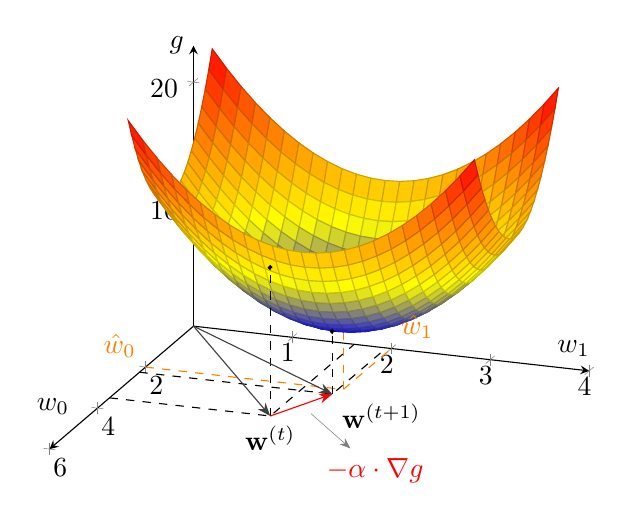
\begin{tikzpicture}
    \begin{axis}[
        grid=major, axis lines=center,
        view={110}{25},
        xmin=0,xmax=+6,
        ymin=0,ymax=+4,
        zmin=0, zmax=23,
        xlabel=$w_0$,
        ylabel=$w_1$,
        zlabel={$g$},
        zlabel style={at={(ticklabel* cs:1)},anchor=east},
        ]
    \draw[dashed,orange](2,2,0)--(2,2,5);
    \addplot3[surf, domain=0.25:3.75, domain y=0.25:3.75] 
        {3*(x-2)^2+3*(y-2)^2+5};
    \draw[dashed,orange](2,0,0)node[above left]{$\hat{w}_0$}--(2,2,0)--(0,2,0)node[above right]{$\hat{w}_1$};
    \draw[dashed](2.25,1.95,0)coordinate(a)node[below right]{$\vect{w}^{(t+1)}$}--(2.25,1.95,5.1275)node[draw, circle, fill=black, inner sep=0.5pt]{};
    \draw[dashed](3.5,1.625,0)coordinate(b)node[below]{$\vect{w}^{(t)}$}--(3.5,1.625,12.171875)node[draw, circle, fill=black, inner sep=0.5pt]{};
    \draw[dashed](3.5,0,0)--(b)--(0,1.625,0);
    \draw[dashed](2.25,0,0)--(a)--(0,1.95,0);
    \draw[-Stealth,darkgray](zticklabel* cs:0,0)--(a);
    \draw[-Stealth,darkgray](zticklabel* cs:0,0)--(b);
    \draw[-Stealth,red](b)--(a)node[midway, pin=290:{$-\alpha\cdot\nabla g$}]{};
    \end{axis}
\end{tikzpicture}
\end{document}